%\documentclass{standalone}
%\usepackage{tikz}
%\usetikzlibrary{patterns,plotmarks}
%\begin{document}
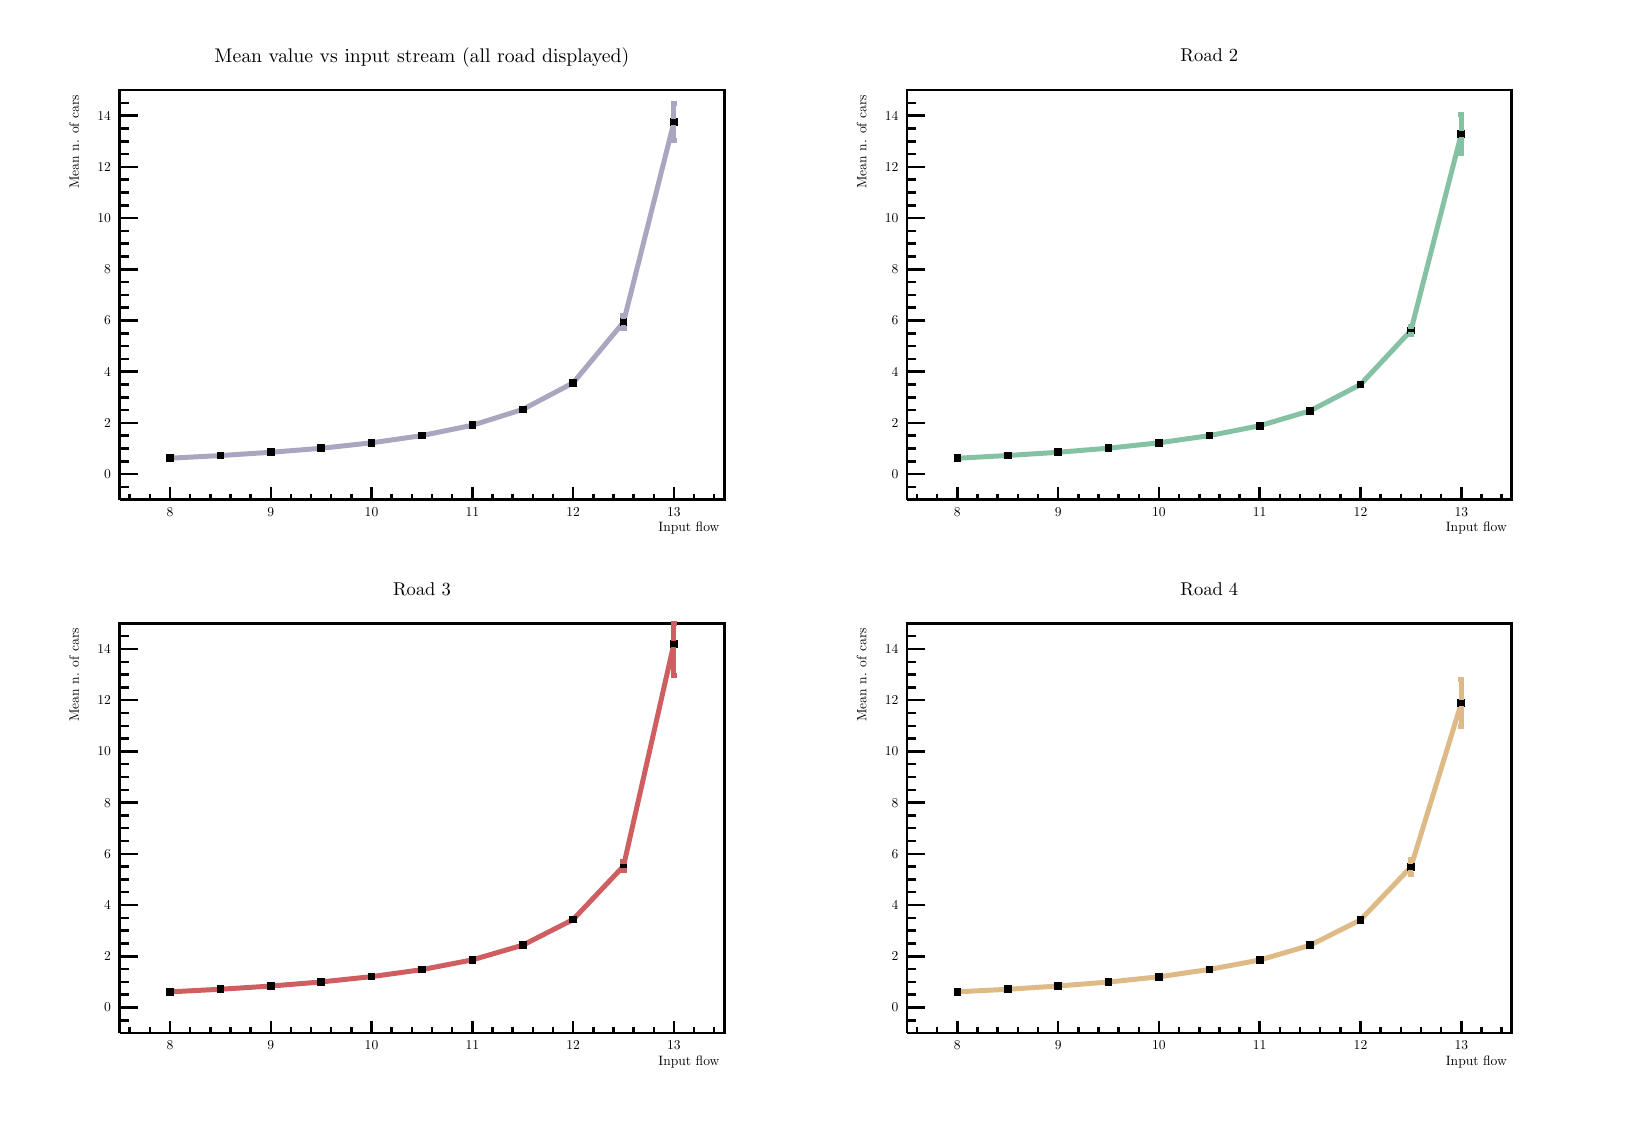
\begin{tikzpicture}
\def\CheckTikzLibraryLoaded#1{ \ifcsname tikz@library@#1@loaded\endcsname \else \PackageWarning{tikz}{usetikzlibrary{#1} is missing in the preamble.} \fi }
\CheckTikzLibraryLoaded{patterns}
\CheckTikzLibraryLoaded{plotmarks}
\pgfdeclareplotmark{cross} {
\pgfpathmoveto{\pgfpoint{-0.3\pgfplotmarksize}{\pgfplotmarksize}}
\pgfpathlineto{\pgfpoint{+0.3\pgfplotmarksize}{\pgfplotmarksize}}
\pgfpathlineto{\pgfpoint{+0.3\pgfplotmarksize}{0.3\pgfplotmarksize}}
\pgfpathlineto{\pgfpoint{+1\pgfplotmarksize}{0.3\pgfplotmarksize}}
\pgfpathlineto{\pgfpoint{+1\pgfplotmarksize}{-0.3\pgfplotmarksize}}
\pgfpathlineto{\pgfpoint{+0.3\pgfplotmarksize}{-0.3\pgfplotmarksize}}
\pgfpathlineto{\pgfpoint{+0.3\pgfplotmarksize}{-1.\pgfplotmarksize}}
\pgfpathlineto{\pgfpoint{-0.3\pgfplotmarksize}{-1.\pgfplotmarksize}}
\pgfpathlineto{\pgfpoint{-0.3\pgfplotmarksize}{-0.3\pgfplotmarksize}}
\pgfpathlineto{\pgfpoint{-1.\pgfplotmarksize}{-0.3\pgfplotmarksize}}
\pgfpathlineto{\pgfpoint{-1.\pgfplotmarksize}{0.3\pgfplotmarksize}}
\pgfpathlineto{\pgfpoint{-0.3\pgfplotmarksize}{0.3\pgfplotmarksize}}
\pgfpathclose
\pgfusepathqstroke
}
\pgfdeclareplotmark{cross*} {
\pgfpathmoveto{\pgfpoint{-0.3\pgfplotmarksize}{\pgfplotmarksize}}
\pgfpathlineto{\pgfpoint{+0.3\pgfplotmarksize}{\pgfplotmarksize}}
\pgfpathlineto{\pgfpoint{+0.3\pgfplotmarksize}{0.3\pgfplotmarksize}}
\pgfpathlineto{\pgfpoint{+1\pgfplotmarksize}{0.3\pgfplotmarksize}}
\pgfpathlineto{\pgfpoint{+1\pgfplotmarksize}{-0.3\pgfplotmarksize}}
\pgfpathlineto{\pgfpoint{+0.3\pgfplotmarksize}{-0.3\pgfplotmarksize}}
\pgfpathlineto{\pgfpoint{+0.3\pgfplotmarksize}{-1.\pgfplotmarksize}}
\pgfpathlineto{\pgfpoint{-0.3\pgfplotmarksize}{-1.\pgfplotmarksize}}
\pgfpathlineto{\pgfpoint{-0.3\pgfplotmarksize}{-0.3\pgfplotmarksize}}
\pgfpathlineto{\pgfpoint{-1.\pgfplotmarksize}{-0.3\pgfplotmarksize}}
\pgfpathlineto{\pgfpoint{-1.\pgfplotmarksize}{0.3\pgfplotmarksize}}
\pgfpathlineto{\pgfpoint{-0.3\pgfplotmarksize}{0.3\pgfplotmarksize}}
\pgfpathclose
\pgfusepathqfillstroke
}
\pgfdeclareplotmark{newstar} {
\pgfpathmoveto{\pgfqpoint{0pt}{\pgfplotmarksize}}
\pgfpathlineto{\pgfqpointpolar{44}{0.5\pgfplotmarksize}}
\pgfpathlineto{\pgfqpointpolar{18}{\pgfplotmarksize}}
\pgfpathlineto{\pgfqpointpolar{-20}{0.5\pgfplotmarksize}}
\pgfpathlineto{\pgfqpointpolar{-54}{\pgfplotmarksize}}
\pgfpathlineto{\pgfqpointpolar{-90}{0.5\pgfplotmarksize}}
\pgfpathlineto{\pgfqpointpolar{234}{\pgfplotmarksize}}
\pgfpathlineto{\pgfqpointpolar{198}{0.5\pgfplotmarksize}}
\pgfpathlineto{\pgfqpointpolar{162}{\pgfplotmarksize}}
\pgfpathlineto{\pgfqpointpolar{134}{0.5\pgfplotmarksize}}
\pgfpathclose
\pgfusepathqstroke
}
\pgfdeclareplotmark{newstar*} {
\pgfpathmoveto{\pgfqpoint{0pt}{\pgfplotmarksize}}
\pgfpathlineto{\pgfqpointpolar{44}{0.5\pgfplotmarksize}}
\pgfpathlineto{\pgfqpointpolar{18}{\pgfplotmarksize}}
\pgfpathlineto{\pgfqpointpolar{-20}{0.5\pgfplotmarksize}}
\pgfpathlineto{\pgfqpointpolar{-54}{\pgfplotmarksize}}
\pgfpathlineto{\pgfqpointpolar{-90}{0.5\pgfplotmarksize}}
\pgfpathlineto{\pgfqpointpolar{234}{\pgfplotmarksize}}
\pgfpathlineto{\pgfqpointpolar{198}{0.5\pgfplotmarksize}}
\pgfpathlineto{\pgfqpointpolar{162}{\pgfplotmarksize}}
\pgfpathlineto{\pgfqpointpolar{134}{0.5\pgfplotmarksize}}
\pgfpathclose
\pgfusepathqfillstroke
}
\definecolor{c}{rgb}{1,1,1};
\draw [color=c, fill=c] (0,0) rectangle (20,13.5471);
\draw [color=c, fill=c] (0.2,6.90902) rectangle (9.8,13.4116);
\draw [color=c, fill=c] (1.16,7.55928) rectangle (8.84,12.7614);
\definecolor{c}{rgb}{0,0,0};
\draw [c,line width=0.9] (1.16,7.55928) -- (1.16,12.7614) -- (8.84,12.7614) -- (8.84,7.55928) -- (1.16,7.55928);
\definecolor{c}{rgb}{1,1,1};
\draw [color=c, fill=c] (1.16,7.55928) rectangle (8.84,12.7614);
\definecolor{c}{rgb}{0,0,0};
\draw [c,line width=0.9] (1.16,7.55928) -- (1.16,12.7614) -- (8.84,12.7614) -- (8.84,7.55928) -- (1.16,7.55928);
\draw [c,line width=0.9] (1.16,7.55928) -- (8.84,7.55928);
\draw [c,line width=0.9] (1.8,7.71534) -- (1.8,7.55928);
\draw [c,line width=0.9] (2.056,7.63731) -- (2.056,7.55928);
\draw [c,line width=0.9] (2.312,7.63731) -- (2.312,7.55928);
\draw [c,line width=0.9] (2.568,7.63731) -- (2.568,7.55928);
\draw [c,line width=0.9] (2.824,7.63731) -- (2.824,7.55928);
\draw [c,line width=0.9] (3.08,7.71534) -- (3.08,7.55928);
\draw [c,line width=0.9] (3.336,7.63731) -- (3.336,7.55928);
\draw [c,line width=0.9] (3.592,7.63731) -- (3.592,7.55928);
\draw [c,line width=0.9] (3.848,7.63731) -- (3.848,7.55928);
\draw [c,line width=0.9] (4.104,7.63731) -- (4.104,7.55928);
\draw [c,line width=0.9] (4.36,7.71534) -- (4.36,7.55928);
\draw [c,line width=0.9] (4.616,7.63731) -- (4.616,7.55928);
\draw [c,line width=0.9] (4.872,7.63731) -- (4.872,7.55928);
\draw [c,line width=0.9] (5.128,7.63731) -- (5.128,7.55928);
\draw [c,line width=0.9] (5.384,7.63731) -- (5.384,7.55928);
\draw [c,line width=0.9] (5.64,7.71534) -- (5.64,7.55928);
\draw [c,line width=0.9] (5.896,7.63731) -- (5.896,7.55928);
\draw [c,line width=0.9] (6.152,7.63731) -- (6.152,7.55928);
\draw [c,line width=0.9] (6.408,7.63731) -- (6.408,7.55928);
\draw [c,line width=0.9] (6.664,7.63731) -- (6.664,7.55928);
\draw [c,line width=0.9] (6.92,7.71534) -- (6.92,7.55928);
\draw [c,line width=0.9] (7.176,7.63731) -- (7.176,7.55928);
\draw [c,line width=0.9] (7.432,7.63731) -- (7.432,7.55928);
\draw [c,line width=0.9] (7.688,7.63731) -- (7.688,7.55928);
\draw [c,line width=0.9] (7.944,7.63731) -- (7.944,7.55928);
\draw [c,line width=0.9] (8.2,7.71534) -- (8.2,7.55928);
\draw [c,line width=0.9] (1.8,7.71534) -- (1.8,7.55928);
\draw [c,line width=0.9] (1.544,7.63731) -- (1.544,7.55928);
\draw [c,line width=0.9] (1.288,7.63731) -- (1.288,7.55928);
\draw [c,line width=0.9] (8.2,7.71534) -- (8.2,7.55928);
\draw [c,line width=0.9] (8.456,7.63731) -- (8.456,7.55928);
\draw [c,line width=0.9] (8.712,7.63731) -- (8.712,7.55928);
\draw [anchor=base] (1.8,7.34469) node[scale=0.490318, color=c, rotate=0]{8};
\draw [anchor=base] (3.08,7.34469) node[scale=0.490318, color=c, rotate=0]{9};
\draw [anchor=base] (4.36,7.34469) node[scale=0.490318, color=c, rotate=0]{10};
\draw [anchor=base] (5.64,7.34469) node[scale=0.490318, color=c, rotate=0]{11};
\draw [anchor=base] (6.92,7.34469) node[scale=0.490318, color=c, rotate=0]{12};
\draw [anchor=base] (8.2,7.34469) node[scale=0.490318, color=c, rotate=0]{13};
\draw [anchor= east] (8.84,7.19513) node[scale=0.490318, color=c, rotate=0]{Input flow};
\draw [c,line width=0.9] (1.16,7.55928) -- (1.16,12.7614);
\draw [c,line width=0.9] (1.3904,7.88441) -- (1.16,7.88441);
\draw [c,line width=0.9] (1.2752,8.04697) -- (1.16,8.04697);
\draw [c,line width=0.9] (1.2752,8.20954) -- (1.16,8.20954);
\draw [c,line width=0.9] (1.2752,8.3721) -- (1.16,8.3721);
\draw [c,line width=0.9] (1.3904,8.53467) -- (1.16,8.53467);
\draw [c,line width=0.9] (1.2752,8.69723) -- (1.16,8.69723);
\draw [c,line width=0.9] (1.2752,8.8598) -- (1.16,8.8598);
\draw [c,line width=0.9] (1.2752,9.02236) -- (1.16,9.02236);
\draw [c,line width=0.9] (1.3904,9.18493) -- (1.16,9.18493);
\draw [c,line width=0.9] (1.2752,9.3475) -- (1.16,9.3475);
\draw [c,line width=0.9] (1.2752,9.51006) -- (1.16,9.51006);
\draw [c,line width=0.9] (1.2752,9.67263) -- (1.16,9.67263);
\draw [c,line width=0.9] (1.3904,9.83519) -- (1.16,9.83519);
\draw [c,line width=0.9] (1.2752,9.99776) -- (1.16,9.99776);
\draw [c,line width=0.9] (1.2752,10.1603) -- (1.16,10.1603);
\draw [c,line width=0.9] (1.2752,10.3229) -- (1.16,10.3229);
\draw [c,line width=0.9] (1.3904,10.4855) -- (1.16,10.4855);
\draw [c,line width=0.9] (1.2752,10.648) -- (1.16,10.648);
\draw [c,line width=0.9] (1.2752,10.8106) -- (1.16,10.8106);
\draw [c,line width=0.9] (1.2752,10.9731) -- (1.16,10.9731);
\draw [c,line width=0.9] (1.3904,11.1357) -- (1.16,11.1357);
\draw [c,line width=0.9] (1.2752,11.2983) -- (1.16,11.2983);
\draw [c,line width=0.9] (1.2752,11.4608) -- (1.16,11.4608);
\draw [c,line width=0.9] (1.2752,11.6234) -- (1.16,11.6234);
\draw [c,line width=0.9] (1.3904,11.786) -- (1.16,11.786);
\draw [c,line width=0.9] (1.2752,11.9485) -- (1.16,11.9485);
\draw [c,line width=0.9] (1.2752,12.1111) -- (1.16,12.1111);
\draw [c,line width=0.9] (1.2752,12.2737) -- (1.16,12.2737);
\draw [c,line width=0.9] (1.3904,12.4362) -- (1.16,12.4362);
\draw [c,line width=0.9] (1.3904,7.88441) -- (1.16,7.88441);
\draw [c,line width=0.9] (1.2752,7.72184) -- (1.16,7.72184);
\draw [c,line width=0.9] (1.2752,7.55928) -- (1.16,7.55928);
\draw [c,line width=0.9] (1.3904,12.4362) -- (1.16,12.4362);
\draw [c,line width=0.9] (1.2752,12.5988) -- (1.16,12.5988);
\draw [c,line width=0.9] (1.2752,12.7614) -- (1.16,12.7614);
\draw [anchor= east] (1.112,7.88441) node[scale=0.490318, color=c, rotate=0]{0};
\draw [anchor= east] (1.112,8.53467) node[scale=0.490318, color=c, rotate=0]{2};
\draw [anchor= east] (1.112,9.18493) node[scale=0.490318, color=c, rotate=0]{4};
\draw [anchor= east] (1.112,9.83519) node[scale=0.490318, color=c, rotate=0]{6};
\draw [anchor= east] (1.112,10.4855) node[scale=0.490318, color=c, rotate=0]{8};
\draw [anchor= east] (1.112,11.1357) node[scale=0.490318, color=c, rotate=0]{10};
\draw [anchor= east] (1.112,11.786) node[scale=0.490318, color=c, rotate=0]{12};
\draw [anchor= east] (1.112,12.4362) node[scale=0.490318, color=c, rotate=0]{14};
\draw [anchor= east] (0.583519,12.7614) node[scale=0.490318, color=c, rotate=90]{Mean n. of cars};
\definecolor{c}{rgb}{0.67,0.65,0.75};
\draw [c,line width=1.8] (1.8,8.08618) -- (2.44,8.11975) -- (3.08,8.1615) -- (3.72,8.2122) -- (4.36,8.28172) -- (5,8.37336) -- (5.64,8.50443) -- (6.28,8.70595) -- (6.92,9.04275) -- (7.56,9.81286) -- (8.2,12.3532);
\definecolor{c}{rgb}{0,0,0};
\foreach \P in {(1.8,8.08618), (2.44,8.11975), (3.08,8.1615), (3.72,8.2122), (4.36,8.28172), (5,8.37336), (5.64,8.50443), (6.28,8.70595), (6.92,9.04275), (7.56,9.81286), (8.2,12.3532)}{\draw[mark options={color=c,fill=c},mark size=1.201201pt, line
 width=0.000000pt, mark=square*] plot coordinates {\P};}
\definecolor{c}{rgb}{0.67,0.65,0.75};
\draw [c,line width=1.8] (7.56,9.85294) -- (7.56,9.89318);
\draw [c,line width=1.8] (7.51992,9.89318) -- (7.60008,9.89318);
\draw [c,line width=1.8] (7.56,9.77278) -- (7.56,9.73254);
\draw [c,line width=1.8] (7.51992,9.73254) -- (7.60008,9.73254);
\draw [c,line width=1.8] (8.2,12.3933) -- (8.2,12.5893);
\draw [c,line width=1.8] (8.15992,12.5893) -- (8.24008,12.5893);
\draw [c,line width=1.8] (8.2,12.3131) -- (8.2,12.1171);
\draw [c,line width=1.8] (8.15992,12.1171) -- (8.24008,12.1171);
\definecolor{c}{rgb}{0,0,0};
\draw (5,13.1747) node[scale=0.71319, color=c, rotate=0]{Mean value vs input stream (all road displayed)};
\definecolor{c}{rgb}{1,1,1};
\draw [color=c, fill=c] (10.2,6.90902) rectangle (19.8,13.4116);
\draw [color=c, fill=c] (11.16,7.55928) rectangle (18.84,12.7614);
\definecolor{c}{rgb}{0,0,0};
\draw [c,line width=0.9] (11.16,7.55928) -- (11.16,12.7614) -- (18.84,12.7614) -- (18.84,7.55928) -- (11.16,7.55928);
\definecolor{c}{rgb}{1,1,1};
\draw [color=c, fill=c] (11.16,7.55928) rectangle (18.84,12.7614);
\definecolor{c}{rgb}{0,0,0};
\draw [c,line width=0.9] (11.16,7.55928) -- (11.16,12.7614) -- (18.84,12.7614) -- (18.84,7.55928) -- (11.16,7.55928);
\draw [c,line width=0.9] (11.16,7.55928) -- (18.84,7.55928);
\draw [c,line width=0.9] (11.8,7.71534) -- (11.8,7.55928);
\draw [c,line width=0.9] (12.056,7.63731) -- (12.056,7.55928);
\draw [c,line width=0.9] (12.312,7.63731) -- (12.312,7.55928);
\draw [c,line width=0.9] (12.568,7.63731) -- (12.568,7.55928);
\draw [c,line width=0.9] (12.824,7.63731) -- (12.824,7.55928);
\draw [c,line width=0.9] (13.08,7.71534) -- (13.08,7.55928);
\draw [c,line width=0.9] (13.336,7.63731) -- (13.336,7.55928);
\draw [c,line width=0.9] (13.592,7.63731) -- (13.592,7.55928);
\draw [c,line width=0.9] (13.848,7.63731) -- (13.848,7.55928);
\draw [c,line width=0.9] (14.104,7.63731) -- (14.104,7.55928);
\draw [c,line width=0.9] (14.36,7.71534) -- (14.36,7.55928);
\draw [c,line width=0.9] (14.616,7.63731) -- (14.616,7.55928);
\draw [c,line width=0.9] (14.872,7.63731) -- (14.872,7.55928);
\draw [c,line width=0.9] (15.128,7.63731) -- (15.128,7.55928);
\draw [c,line width=0.9] (15.384,7.63731) -- (15.384,7.55928);
\draw [c,line width=0.9] (15.64,7.71534) -- (15.64,7.55928);
\draw [c,line width=0.9] (15.896,7.63731) -- (15.896,7.55928);
\draw [c,line width=0.9] (16.152,7.63731) -- (16.152,7.55928);
\draw [c,line width=0.9] (16.408,7.63731) -- (16.408,7.55928);
\draw [c,line width=0.9] (16.664,7.63731) -- (16.664,7.55928);
\draw [c,line width=0.9] (16.92,7.71534) -- (16.92,7.55928);
\draw [c,line width=0.9] (17.176,7.63731) -- (17.176,7.55928);
\draw [c,line width=0.9] (17.432,7.63731) -- (17.432,7.55928);
\draw [c,line width=0.9] (17.688,7.63731) -- (17.688,7.55928);
\draw [c,line width=0.9] (17.944,7.63731) -- (17.944,7.55928);
\draw [c,line width=0.9] (18.2,7.71534) -- (18.2,7.55928);
\draw [c,line width=0.9] (11.8,7.71534) -- (11.8,7.55928);
\draw [c,line width=0.9] (11.544,7.63731) -- (11.544,7.55928);
\draw [c,line width=0.9] (11.288,7.63731) -- (11.288,7.55928);
\draw [c,line width=0.9] (18.2,7.71534) -- (18.2,7.55928);
\draw [c,line width=0.9] (18.456,7.63731) -- (18.456,7.55928);
\draw [c,line width=0.9] (18.712,7.63731) -- (18.712,7.55928);
\draw [anchor=base] (11.8,7.34469) node[scale=0.490318, color=c, rotate=0]{8};
\draw [anchor=base] (13.08,7.34469) node[scale=0.490318, color=c, rotate=0]{9};
\draw [anchor=base] (14.36,7.34469) node[scale=0.490318, color=c, rotate=0]{10};
\draw [anchor=base] (15.64,7.34469) node[scale=0.490318, color=c, rotate=0]{11};
\draw [anchor=base] (16.92,7.34469) node[scale=0.490318, color=c, rotate=0]{12};
\draw [anchor=base] (18.2,7.34469) node[scale=0.490318, color=c, rotate=0]{13};
\draw [anchor= east] (18.84,7.19513) node[scale=0.490318, color=c, rotate=0]{Input flow};
\draw [c,line width=0.9] (11.16,7.55928) -- (11.16,12.7614);
\draw [c,line width=0.9] (11.3904,7.88441) -- (11.16,7.88441);
\draw [c,line width=0.9] (11.2752,8.04697) -- (11.16,8.04697);
\draw [c,line width=0.9] (11.2752,8.20954) -- (11.16,8.20954);
\draw [c,line width=0.9] (11.2752,8.3721) -- (11.16,8.3721);
\draw [c,line width=0.9] (11.3904,8.53467) -- (11.16,8.53467);
\draw [c,line width=0.9] (11.2752,8.69723) -- (11.16,8.69723);
\draw [c,line width=0.9] (11.2752,8.8598) -- (11.16,8.8598);
\draw [c,line width=0.9] (11.2752,9.02236) -- (11.16,9.02236);
\draw [c,line width=0.9] (11.3904,9.18493) -- (11.16,9.18493);
\draw [c,line width=0.9] (11.2752,9.3475) -- (11.16,9.3475);
\draw [c,line width=0.9] (11.2752,9.51006) -- (11.16,9.51006);
\draw [c,line width=0.9] (11.2752,9.67263) -- (11.16,9.67263);
\draw [c,line width=0.9] (11.3904,9.83519) -- (11.16,9.83519);
\draw [c,line width=0.9] (11.2752,9.99776) -- (11.16,9.99776);
\draw [c,line width=0.9] (11.2752,10.1603) -- (11.16,10.1603);
\draw [c,line width=0.9] (11.2752,10.3229) -- (11.16,10.3229);
\draw [c,line width=0.9] (11.3904,10.4855) -- (11.16,10.4855);
\draw [c,line width=0.9] (11.2752,10.648) -- (11.16,10.648);
\draw [c,line width=0.9] (11.2752,10.8106) -- (11.16,10.8106);
\draw [c,line width=0.9] (11.2752,10.9731) -- (11.16,10.9731);
\draw [c,line width=0.9] (11.3904,11.1357) -- (11.16,11.1357);
\draw [c,line width=0.9] (11.2752,11.2983) -- (11.16,11.2983);
\draw [c,line width=0.9] (11.2752,11.4608) -- (11.16,11.4608);
\draw [c,line width=0.9] (11.2752,11.6234) -- (11.16,11.6234);
\draw [c,line width=0.9] (11.3904,11.786) -- (11.16,11.786);
\draw [c,line width=0.9] (11.2752,11.9485) -- (11.16,11.9485);
\draw [c,line width=0.9] (11.2752,12.1111) -- (11.16,12.1111);
\draw [c,line width=0.9] (11.2752,12.2737) -- (11.16,12.2737);
\draw [c,line width=0.9] (11.3904,12.4362) -- (11.16,12.4362);
\draw [c,line width=0.9] (11.3904,7.88441) -- (11.16,7.88441);
\draw [c,line width=0.9] (11.2752,7.72184) -- (11.16,7.72184);
\draw [c,line width=0.9] (11.2752,7.55928) -- (11.16,7.55928);
\draw [c,line width=0.9] (11.3904,12.4362) -- (11.16,12.4362);
\draw [c,line width=0.9] (11.2752,12.5988) -- (11.16,12.5988);
\draw [c,line width=0.9] (11.2752,12.7614) -- (11.16,12.7614);
\draw [anchor= east] (11.112,7.88441) node[scale=0.490318, color=c, rotate=0]{0};
\draw [anchor= east] (11.112,8.53467) node[scale=0.490318, color=c, rotate=0]{2};
\draw [anchor= east] (11.112,9.18493) node[scale=0.490318, color=c, rotate=0]{4};
\draw [anchor= east] (11.112,9.83519) node[scale=0.490318, color=c, rotate=0]{6};
\draw [anchor= east] (11.112,10.4855) node[scale=0.490318, color=c, rotate=0]{8};
\draw [anchor= east] (11.112,11.1357) node[scale=0.490318, color=c, rotate=0]{10};
\draw [anchor= east] (11.112,11.786) node[scale=0.490318, color=c, rotate=0]{12};
\draw [anchor= east] (11.112,12.4362) node[scale=0.490318, color=c, rotate=0]{14};
\draw [anchor= east] (10.5835,12.7614) node[scale=0.490318, color=c, rotate=90]{Mean n. of cars};
\definecolor{c}{rgb}{0.52,0.76,0.64};
\draw [c,line width=1.8] (11.8,8.08559) -- (12.44,8.12075) -- (13.08,8.16133) -- (13.72,8.21364) -- (14.36,8.2816) -- (15,8.37269) -- (15.64,8.49878) -- (16.28,8.68806) -- (16.92,9.02238) -- (17.56,9.70748) -- (18.2,12.2063);
\definecolor{c}{rgb}{0,0,0};
\foreach \P in {(11.8,8.08559), (12.44,8.12075), (13.08,8.16133), (13.72,8.21364), (14.36,8.2816), (15,8.37269), (15.64,8.49878), (16.28,8.68806), (16.92,9.02238), (17.56,9.70748), (18.2,12.2063)}{\draw[mark options={color=c,fill=c},mark
 size=1.201201pt, line width=0.000000pt, mark=square*] plot coordinates {\P};}
\definecolor{c}{rgb}{0.52,0.76,0.64};
\draw [c,line width=1.8] (17.56,9.74756) -- (17.56,9.76356);
\draw [c,line width=1.8] (17.5199,9.76356) -- (17.6001,9.76356);
\draw [c,line width=1.8] (17.56,9.6674) -- (17.56,9.6514);
\draw [c,line width=1.8] (17.5199,9.6514) -- (17.6001,9.6514);
\draw [c,line width=1.8] (18.2,12.2464) -- (18.2,12.4562);
\draw [c,line width=1.8] (18.1599,12.4562) -- (18.2401,12.4562);
\draw [c,line width=1.8] (18.2,12.1662) -- (18.2,11.9563);
\draw [c,line width=1.8] (18.1599,11.9563) -- (18.2401,11.9563);
\definecolor{c}{rgb}{0,0,0};
\draw (15,13.2003) node[scale=0.668615, color=c, rotate=0]{Road 2};
\definecolor{c}{rgb}{1,1,1};
\draw [color=c, fill=c] (0.2,0.135471) rectangle (9.8,6.63808);
\draw [color=c, fill=c] (1.16,0.785731) rectangle (8.84,5.98782);
\definecolor{c}{rgb}{0,0,0};
\draw [c,line width=0.9] (1.16,0.785731) -- (1.16,5.98782) -- (8.84,5.98782) -- (8.84,0.785731) -- (1.16,0.785731);
\definecolor{c}{rgb}{1,1,1};
\draw [color=c, fill=c] (1.16,0.785731) rectangle (8.84,5.98782);
\definecolor{c}{rgb}{0,0,0};
\draw [c,line width=0.9] (1.16,0.785731) -- (1.16,5.98782) -- (8.84,5.98782) -- (8.84,0.785731) -- (1.16,0.785731);
\draw [c,line width=0.9] (1.16,0.785731) -- (8.84,0.785731);
\draw [c,line width=0.9] (1.8,0.941794) -- (1.8,0.785731);
\draw [c,line width=0.9] (2.056,0.863763) -- (2.056,0.785731);
\draw [c,line width=0.9] (2.312,0.863763) -- (2.312,0.785731);
\draw [c,line width=0.9] (2.568,0.863763) -- (2.568,0.785731);
\draw [c,line width=0.9] (2.824,0.863763) -- (2.824,0.785731);
\draw [c,line width=0.9] (3.08,0.941794) -- (3.08,0.785731);
\draw [c,line width=0.9] (3.336,0.863763) -- (3.336,0.785731);
\draw [c,line width=0.9] (3.592,0.863763) -- (3.592,0.785731);
\draw [c,line width=0.9] (3.848,0.863763) -- (3.848,0.785731);
\draw [c,line width=0.9] (4.104,0.863763) -- (4.104,0.785731);
\draw [c,line width=0.9] (4.36,0.941794) -- (4.36,0.785731);
\draw [c,line width=0.9] (4.616,0.863763) -- (4.616,0.785731);
\draw [c,line width=0.9] (4.872,0.863763) -- (4.872,0.785731);
\draw [c,line width=0.9] (5.128,0.863763) -- (5.128,0.785731);
\draw [c,line width=0.9] (5.384,0.863763) -- (5.384,0.785731);
\draw [c,line width=0.9] (5.64,0.941794) -- (5.64,0.785731);
\draw [c,line width=0.9] (5.896,0.863763) -- (5.896,0.785731);
\draw [c,line width=0.9] (6.152,0.863763) -- (6.152,0.785731);
\draw [c,line width=0.9] (6.408,0.863763) -- (6.408,0.785731);
\draw [c,line width=0.9] (6.664,0.863763) -- (6.664,0.785731);
\draw [c,line width=0.9] (6.92,0.941794) -- (6.92,0.785731);
\draw [c,line width=0.9] (7.176,0.863763) -- (7.176,0.785731);
\draw [c,line width=0.9] (7.432,0.863763) -- (7.432,0.785731);
\draw [c,line width=0.9] (7.688,0.863763) -- (7.688,0.785731);
\draw [c,line width=0.9] (7.944,0.863763) -- (7.944,0.785731);
\draw [c,line width=0.9] (8.2,0.941794) -- (8.2,0.785731);
\draw [c,line width=0.9] (1.8,0.941794) -- (1.8,0.785731);
\draw [c,line width=0.9] (1.544,0.863763) -- (1.544,0.785731);
\draw [c,line width=0.9] (1.288,0.863763) -- (1.288,0.785731);
\draw [c,line width=0.9] (8.2,0.941794) -- (8.2,0.785731);
\draw [c,line width=0.9] (8.456,0.863763) -- (8.456,0.785731);
\draw [c,line width=0.9] (8.712,0.863763) -- (8.712,0.785731);
\draw [anchor=base] (1.8,0.571146) node[scale=0.490318, color=c, rotate=0]{8};
\draw [anchor=base] (3.08,0.571146) node[scale=0.490318, color=c, rotate=0]{9};
\draw [anchor=base] (4.36,0.571146) node[scale=0.490318, color=c, rotate=0]{10};
\draw [anchor=base] (5.64,0.571146) node[scale=0.490318, color=c, rotate=0]{11};
\draw [anchor=base] (6.92,0.571146) node[scale=0.490318, color=c, rotate=0]{12};
\draw [anchor=base] (8.2,0.571146) node[scale=0.490318, color=c, rotate=0]{13};
\draw [anchor= east] (8.84,0.421586) node[scale=0.490318, color=c, rotate=0]{Input flow};
\draw [c,line width=0.9] (1.16,0.785731) -- (1.16,5.98782);
\draw [c,line width=0.9] (1.3904,1.11086) -- (1.16,1.11086);
\draw [c,line width=0.9] (1.2752,1.27343) -- (1.16,1.27343);
\draw [c,line width=0.9] (1.2752,1.43599) -- (1.16,1.43599);
\draw [c,line width=0.9] (1.2752,1.59856) -- (1.16,1.59856);
\draw [c,line width=0.9] (1.3904,1.76112) -- (1.16,1.76112);
\draw [c,line width=0.9] (1.2752,1.92369) -- (1.16,1.92369);
\draw [c,line width=0.9] (1.2752,2.08625) -- (1.16,2.08625);
\draw [c,line width=0.9] (1.2752,2.24882) -- (1.16,2.24882);
\draw [c,line width=0.9] (1.3904,2.41138) -- (1.16,2.41138);
\draw [c,line width=0.9] (1.2752,2.57395) -- (1.16,2.57395);
\draw [c,line width=0.9] (1.2752,2.73651) -- (1.16,2.73651);
\draw [c,line width=0.9] (1.2752,2.89908) -- (1.16,2.89908);
\draw [c,line width=0.9] (1.3904,3.06164) -- (1.16,3.06164);
\draw [c,line width=0.9] (1.2752,3.22421) -- (1.16,3.22421);
\draw [c,line width=0.9] (1.2752,3.38677) -- (1.16,3.38677);
\draw [c,line width=0.9] (1.2752,3.54934) -- (1.16,3.54934);
\draw [c,line width=0.9] (1.3904,3.7119) -- (1.16,3.7119);
\draw [c,line width=0.9] (1.2752,3.87447) -- (1.16,3.87447);
\draw [c,line width=0.9] (1.2752,4.03703) -- (1.16,4.03703);
\draw [c,line width=0.9] (1.2752,4.1996) -- (1.16,4.1996);
\draw [c,line width=0.9] (1.3904,4.36216) -- (1.16,4.36216);
\draw [c,line width=0.9] (1.2752,4.52473) -- (1.16,4.52473);
\draw [c,line width=0.9] (1.2752,4.68729) -- (1.16,4.68729);
\draw [c,line width=0.9] (1.2752,4.84986) -- (1.16,4.84986);
\draw [c,line width=0.9] (1.3904,5.01242) -- (1.16,5.01242);
\draw [c,line width=0.9] (1.2752,5.17499) -- (1.16,5.17499);
\draw [c,line width=0.9] (1.2752,5.33755) -- (1.16,5.33755);
\draw [c,line width=0.9] (1.2752,5.50012) -- (1.16,5.50012);
\draw [c,line width=0.9] (1.3904,5.66269) -- (1.16,5.66269);
\draw [c,line width=0.9] (1.3904,1.11086) -- (1.16,1.11086);
\draw [c,line width=0.9] (1.2752,0.948297) -- (1.16,0.948297);
\draw [c,line width=0.9] (1.2752,0.785731) -- (1.16,0.785731);
\draw [c,line width=0.9] (1.3904,5.66269) -- (1.16,5.66269);
\draw [c,line width=0.9] (1.2752,5.82525) -- (1.16,5.82525);
\draw [c,line width=0.9] (1.2752,5.98782) -- (1.16,5.98782);
\draw [anchor= east] (1.112,1.11086) node[scale=0.490318, color=c, rotate=0]{0};
\draw [anchor= east] (1.112,1.76112) node[scale=0.490318, color=c, rotate=0]{2};
\draw [anchor= east] (1.112,2.41138) node[scale=0.490318, color=c, rotate=0]{4};
\draw [anchor= east] (1.112,3.06164) node[scale=0.490318, color=c, rotate=0]{6};
\draw [anchor= east] (1.112,3.7119) node[scale=0.490318, color=c, rotate=0]{8};
\draw [anchor= east] (1.112,4.36216) node[scale=0.490318, color=c, rotate=0]{10};
\draw [anchor= east] (1.112,5.01242) node[scale=0.490318, color=c, rotate=0]{12};
\draw [anchor= east] (1.112,5.66269) node[scale=0.490318, color=c, rotate=0]{14};
\draw [anchor= east] (0.583519,5.98782) node[scale=0.490318, color=c, rotate=90]{Mean n. of cars};
\definecolor{c}{rgb}{0.81,0.37,0.38};
\draw [c,line width=1.8] (1.8,1.30879) -- (2.44,1.34227) -- (3.08,1.38238) -- (3.72,1.43485) -- (4.36,1.50224) -- (5,1.59122) -- (5.64,1.71521) -- (6.28,1.90196) -- (6.92,2.22726) -- (7.56,2.90559) -- (8.2,5.73036);
\definecolor{c}{rgb}{0,0,0};
\foreach \P in {(1.8,1.30879), (2.44,1.34227), (3.08,1.38238), (3.72,1.43485), (4.36,1.50224), (5,1.59122), (5.64,1.71521), (6.28,1.90196), (6.92,2.22726), (7.56,2.90559), (8.2,5.73036)}{\draw[mark options={color=c,fill=c},mark size=1.201201pt, line
 width=0.000000pt, mark=square*] plot coordinates {\P};}
\definecolor{c}{rgb}{0.81,0.37,0.38};
\draw [c,line width=1.8] (7.56,2.94567) -- (7.56,2.96401);
\draw [c,line width=1.8] (7.51992,2.96401) -- (7.60008,2.96401);
\draw [c,line width=1.8] (7.56,2.86551) -- (7.56,2.84716);
\draw [c,line width=1.8] (7.51992,2.84716) -- (7.60008,2.84716);
\draw [c,line width=1.8] (8.2,5.77044) -- (8.2,5.98782);
\draw [c,line width=1.8] (8.15992,5.98782) -- (8.24008,5.98782);
\draw [c,line width=1.8] (8.2,5.69028) -- (8.2,5.32216);
\draw [c,line width=1.8] (8.15992,5.32216) -- (8.24008,5.32216);
\definecolor{c}{rgb}{0,0,0};
\draw (5,6.42674) node[scale=0.668615, color=c, rotate=0]{Road 3};
\definecolor{c}{rgb}{1,1,1};
\draw [color=c, fill=c] (10.2,0.135471) rectangle (19.8,6.63808);
\draw [color=c, fill=c] (11.16,0.785731) rectangle (18.84,5.98782);
\definecolor{c}{rgb}{0,0,0};
\draw [c,line width=0.9] (11.16,0.785731) -- (11.16,5.98782) -- (18.84,5.98782) -- (18.84,0.785731) -- (11.16,0.785731);
\definecolor{c}{rgb}{1,1,1};
\draw [color=c, fill=c] (11.16,0.785731) rectangle (18.84,5.98782);
\definecolor{c}{rgb}{0,0,0};
\draw [c,line width=0.9] (11.16,0.785731) -- (11.16,5.98782) -- (18.84,5.98782) -- (18.84,0.785731) -- (11.16,0.785731);
\draw [c,line width=0.9] (11.16,0.785731) -- (18.84,0.785731);
\draw [c,line width=0.9] (11.8,0.941794) -- (11.8,0.785731);
\draw [c,line width=0.9] (12.056,0.863763) -- (12.056,0.785731);
\draw [c,line width=0.9] (12.312,0.863763) -- (12.312,0.785731);
\draw [c,line width=0.9] (12.568,0.863763) -- (12.568,0.785731);
\draw [c,line width=0.9] (12.824,0.863763) -- (12.824,0.785731);
\draw [c,line width=0.9] (13.08,0.941794) -- (13.08,0.785731);
\draw [c,line width=0.9] (13.336,0.863763) -- (13.336,0.785731);
\draw [c,line width=0.9] (13.592,0.863763) -- (13.592,0.785731);
\draw [c,line width=0.9] (13.848,0.863763) -- (13.848,0.785731);
\draw [c,line width=0.9] (14.104,0.863763) -- (14.104,0.785731);
\draw [c,line width=0.9] (14.36,0.941794) -- (14.36,0.785731);
\draw [c,line width=0.9] (14.616,0.863763) -- (14.616,0.785731);
\draw [c,line width=0.9] (14.872,0.863763) -- (14.872,0.785731);
\draw [c,line width=0.9] (15.128,0.863763) -- (15.128,0.785731);
\draw [c,line width=0.9] (15.384,0.863763) -- (15.384,0.785731);
\draw [c,line width=0.9] (15.64,0.941794) -- (15.64,0.785731);
\draw [c,line width=0.9] (15.896,0.863763) -- (15.896,0.785731);
\draw [c,line width=0.9] (16.152,0.863763) -- (16.152,0.785731);
\draw [c,line width=0.9] (16.408,0.863763) -- (16.408,0.785731);
\draw [c,line width=0.9] (16.664,0.863763) -- (16.664,0.785731);
\draw [c,line width=0.9] (16.92,0.941794) -- (16.92,0.785731);
\draw [c,line width=0.9] (17.176,0.863763) -- (17.176,0.785731);
\draw [c,line width=0.9] (17.432,0.863763) -- (17.432,0.785731);
\draw [c,line width=0.9] (17.688,0.863763) -- (17.688,0.785731);
\draw [c,line width=0.9] (17.944,0.863763) -- (17.944,0.785731);
\draw [c,line width=0.9] (18.2,0.941794) -- (18.2,0.785731);
\draw [c,line width=0.9] (11.8,0.941794) -- (11.8,0.785731);
\draw [c,line width=0.9] (11.544,0.863763) -- (11.544,0.785731);
\draw [c,line width=0.9] (11.288,0.863763) -- (11.288,0.785731);
\draw [c,line width=0.9] (18.2,0.941794) -- (18.2,0.785731);
\draw [c,line width=0.9] (18.456,0.863763) -- (18.456,0.785731);
\draw [c,line width=0.9] (18.712,0.863763) -- (18.712,0.785731);
\draw [anchor=base] (11.8,0.571146) node[scale=0.490318, color=c, rotate=0]{8};
\draw [anchor=base] (13.08,0.571146) node[scale=0.490318, color=c, rotate=0]{9};
\draw [anchor=base] (14.36,0.571146) node[scale=0.490318, color=c, rotate=0]{10};
\draw [anchor=base] (15.64,0.571146) node[scale=0.490318, color=c, rotate=0]{11};
\draw [anchor=base] (16.92,0.571146) node[scale=0.490318, color=c, rotate=0]{12};
\draw [anchor=base] (18.2,0.571146) node[scale=0.490318, color=c, rotate=0]{13};
\draw [anchor= east] (18.84,0.421586) node[scale=0.490318, color=c, rotate=0]{Input flow};
\draw [c,line width=0.9] (11.16,0.785731) -- (11.16,5.98782);
\draw [c,line width=0.9] (11.3904,1.11086) -- (11.16,1.11086);
\draw [c,line width=0.9] (11.2752,1.27343) -- (11.16,1.27343);
\draw [c,line width=0.9] (11.2752,1.43599) -- (11.16,1.43599);
\draw [c,line width=0.9] (11.2752,1.59856) -- (11.16,1.59856);
\draw [c,line width=0.9] (11.3904,1.76112) -- (11.16,1.76112);
\draw [c,line width=0.9] (11.2752,1.92369) -- (11.16,1.92369);
\draw [c,line width=0.9] (11.2752,2.08625) -- (11.16,2.08625);
\draw [c,line width=0.9] (11.2752,2.24882) -- (11.16,2.24882);
\draw [c,line width=0.9] (11.3904,2.41138) -- (11.16,2.41138);
\draw [c,line width=0.9] (11.2752,2.57395) -- (11.16,2.57395);
\draw [c,line width=0.9] (11.2752,2.73651) -- (11.16,2.73651);
\draw [c,line width=0.9] (11.2752,2.89908) -- (11.16,2.89908);
\draw [c,line width=0.9] (11.3904,3.06164) -- (11.16,3.06164);
\draw [c,line width=0.9] (11.2752,3.22421) -- (11.16,3.22421);
\draw [c,line width=0.9] (11.2752,3.38677) -- (11.16,3.38677);
\draw [c,line width=0.9] (11.2752,3.54934) -- (11.16,3.54934);
\draw [c,line width=0.9] (11.3904,3.7119) -- (11.16,3.7119);
\draw [c,line width=0.9] (11.2752,3.87447) -- (11.16,3.87447);
\draw [c,line width=0.9] (11.2752,4.03703) -- (11.16,4.03703);
\draw [c,line width=0.9] (11.2752,4.1996) -- (11.16,4.1996);
\draw [c,line width=0.9] (11.3904,4.36216) -- (11.16,4.36216);
\draw [c,line width=0.9] (11.2752,4.52473) -- (11.16,4.52473);
\draw [c,line width=0.9] (11.2752,4.68729) -- (11.16,4.68729);
\draw [c,line width=0.9] (11.2752,4.84986) -- (11.16,4.84986);
\draw [c,line width=0.9] (11.3904,5.01242) -- (11.16,5.01242);
\draw [c,line width=0.9] (11.2752,5.17499) -- (11.16,5.17499);
\draw [c,line width=0.9] (11.2752,5.33755) -- (11.16,5.33755);
\draw [c,line width=0.9] (11.2752,5.50012) -- (11.16,5.50012);
\draw [c,line width=0.9] (11.3904,5.66269) -- (11.16,5.66269);
\draw [c,line width=0.9] (11.3904,1.11086) -- (11.16,1.11086);
\draw [c,line width=0.9] (11.2752,0.948297) -- (11.16,0.948297);
\draw [c,line width=0.9] (11.2752,0.785731) -- (11.16,0.785731);
\draw [c,line width=0.9] (11.3904,5.66269) -- (11.16,5.66269);
\draw [c,line width=0.9] (11.2752,5.82525) -- (11.16,5.82525);
\draw [c,line width=0.9] (11.2752,5.98782) -- (11.16,5.98782);
\draw [anchor= east] (11.112,1.11086) node[scale=0.490318, color=c, rotate=0]{0};
\draw [anchor= east] (11.112,1.76112) node[scale=0.490318, color=c, rotate=0]{2};
\draw [anchor= east] (11.112,2.41138) node[scale=0.490318, color=c, rotate=0]{4};
\draw [anchor= east] (11.112,3.06164) node[scale=0.490318, color=c, rotate=0]{6};
\draw [anchor= east] (11.112,3.7119) node[scale=0.490318, color=c, rotate=0]{8};
\draw [anchor= east] (11.112,4.36216) node[scale=0.490318, color=c, rotate=0]{10};
\draw [anchor= east] (11.112,5.01242) node[scale=0.490318, color=c, rotate=0]{12};
\draw [anchor= east] (11.112,5.66269) node[scale=0.490318, color=c, rotate=0]{14};
\draw [anchor= east] (10.5835,5.98782) node[scale=0.490318, color=c, rotate=90]{Mean n. of cars};
\definecolor{c}{rgb}{0.87,0.73,0.53};
\draw [c,line width=1.8] (11.8,1.30935) -- (12.44,1.34168) -- (13.08,1.38325) -- (13.72,1.43365) -- (14.36,1.50015) -- (15,1.59366) -- (15.64,1.7132) -- (16.28,1.90049) -- (16.92,2.22254) -- (17.56,2.89441) -- (18.2,4.97516);
\definecolor{c}{rgb}{0,0,0};
\foreach \P in {(11.8,1.30935), (12.44,1.34168), (13.08,1.38325), (13.72,1.43365), (14.36,1.50015), (15,1.59366), (15.64,1.7132), (16.28,1.90049), (16.92,2.22254), (17.56,2.89441), (18.2,4.97516)}{\draw[mark options={color=c,fill=c},mark
 size=1.201201pt, line width=0.000000pt, mark=square*] plot coordinates {\P};}
\definecolor{c}{rgb}{0.87,0.73,0.53};
\draw [c,line width=1.8] (17.56,2.93449) -- (17.56,2.99429);
\draw [c,line width=1.8] (17.5199,2.99429) -- (17.6001,2.99429);
\draw [c,line width=1.8] (17.56,2.85433) -- (17.56,2.79454);
\draw [c,line width=1.8] (17.5199,2.79454) -- (17.6001,2.79454);
\draw [c,line width=1.8] (18.2,5.01524) -- (18.2,5.27628);
\draw [c,line width=1.8] (18.1599,5.27628) -- (18.2401,5.27628);
\draw [c,line width=1.8] (18.2,4.93508) -- (18.2,4.67405);
\draw [c,line width=1.8] (18.1599,4.67405) -- (18.2401,4.67405);
\definecolor{c}{rgb}{0,0,0};
\draw (15,6.42674) node[scale=0.668615, color=c, rotate=0]{Road 4};
\end{tikzpicture}
%\end{document}
